
% This work is licensed under the Creative Commons Attribution-Share Alike 2.0 France License.
% To view a copy of this license, visit http://creativecommons.org/licenses/by-sa/2.0/fr/legalcode
% or send a letter to Creative Commons, 171 Second Street, Suite 300, San Francisco, California, 94105, USA.



\chapter{Encore et encore}
\section{Rabâchage}
Il n'y pas grand chose de pire que de faire la même chose encore et encore\footnote{\url{http://fr.wikipedia.org/wiki/Sisyphe}}.
C'est la raison pour laquelle vos parents vous disent de compter les moutons pour essayer de dormir et cela n'a rien avoir avec les incroyables pouvoirs somnifères des mammifères laineux. Cela  a tout avoir avec le fait que répéter quelque chose sans fin est ennuyeux, et que votre esprit devrait tomber dans le sommeil plus facilement s'il n'est pas en train de se concentrer sur quelque chose d'intéressant.\\


Les programmeurs, eux aussi, n'aiment pas particulièrement répéter les choses. Cela les endort aussi. C'est la vraie raison pour laquelle tous les langages de programmation de haut niveau\footnote{Les boucles ont été introduites avec le langage Fortran en 1958.} ont quelque chose appelé une boucle. Par exemple pour afficher «~hello~»  cinq fois en Python vous pouvez faire comme suit:

\begin{Verbatim}[frame=single,rulecolor=\color{gray}, label=ne pas saisir]
>>> print("hello")
hello
>>> print("hello")
hello
>>> print("hello")
hello
>>> print("hello")
hello
>>> print("hello")
hello
\end{Verbatim}

\emph{Ce qui est... Plutôt ennuyant, pour être poli.}\\


Ou nous pouvons utiliser une boucle:

\begin{Verbatim}[frame=single,rulecolor=\color{green}, label=à taper avec attention]
>>> for x in range(0, 5):
...     print('hello')
...
hello
hello
hello
hello
hello
\end{Verbatim}

Comme au chapitre précédent les espaces sont importants, je vous les montre de manière plus explicite avec des arobases:

\begin{Verbatim}[frame=single,rulecolor=\color{gray}, label=ne pas saisir]
>>> for x in range(0, 5):
... @@@@print('hello')
...
\end{Verbatim}

Le mot \emph{for} signifie «~pour~»  en anglais, \emph{in} signifie «~dans~» et \emph{range} signifie gamme (de produit), éventail (de valeurs), série (de valeurs).

La fonction «~\texttt{range}~» permet de créer facilement et rapidement une liste (une série) de nombre entre un début et une fin, par exemple:

\begin{Verbatim}[frame=single,rulecolor=\color{mbleu}, label=à taper]
>>> print(list(range(10, 20)))
[10, 11, 12, 13, 14, 15, 16, 17, 18, 19]
\end{Verbatim}

Si nous ne fournissons qu'un nombre à «~\texttt{range}~» la liste part de zéro («~\texttt{range(n) == range(0,n)}~»:

\begin{Verbatim}[frame=single,rulecolor=\color{mbleu}, label=à taper]
>>> print(list(range(5)))
[0, 1, 2, 3, 4]
\end{Verbatim}

Le mot \emph{list} signifie liste (oui je sais vous aviez deviné).

Dans le cas de Python la boucle utilisée s'appelle un itérateur. Le code «~\texttt{for x in range(0,5)}~» dit en fait à Python de créer une liste de nombre (0, 1, 2, 3, 4) puis pour chacun de ces nombres de stocker cette valeur dans la variable «~\texttt{x}~» et enfin d'exécuter la commande dans le bloc après les deux points pour chaque valeur de «~\texttt{x}~». Nous pouvons utiliser ce «~\texttt{x}~»  dans notre déclaration qui contient «~\texttt{print}~» si nous le voulons:

\begin{Verbatim}[frame=single,rulecolor=\color{green}, label=à taper avec attention]
>>> for x in range(0, 5):
...     print('hello %s' % x)
hello 0
hello 1
hello 2
hello 3
hello 4
\end{Verbatim}

Une représentation graphique peut être observée figure \ref{fig:for}.
\begin{figure}[ht]
\centering
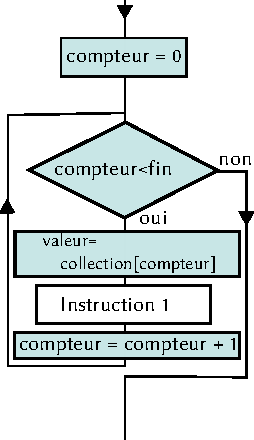
\includegraphics[scale=1.5]{images/for.pdf}
\caption{Diagramme d'un itérateur}
\label{fig:for}
\end{figure}

Si nous déroulions la boucle que nous venons d'éxécuter, cela pourrait ressembler à quelque chose comme cela:

\begin{Verbatim}[frame=single,rulecolor=\color{gray}, label=ne pas saisir]
x = 0
print('hello %s' % x)
x = 1
print('hello %s' % x)
x = 2
print('hello %s' % x)
x = 3
print('hello %s' % x)
x = 4
print('hello %s' % x)
\end{Verbatim}

Ainsi cette boucle (cet itérateur) nous a épargné d'écrire huit lignes de code supplémentaires. C'est vraiment utile, d'autant plus que le programmeur moyen est plus encore paresseux qu'un hippopotame (un jour chaud) quand il s'agit de taper quelque chose. Les bons programmeurs détestent faire les choses plus d'une fois, donc les boucles sont une des structures les plus utiles dans un langage de programmation.\\

Nous n'avons pas obligation d'utiliser «~\texttt{range}~», nous pouvons utiliser les listes que nous avons déjà utilisées:

\begin{small}
\begin{Verbatim}[frame=single,rulecolor=\color{green}, label=à taper avec attention]
>>> courses=['lait', 'fromage', 'laitue', 'confiture', 'sirop', 'chocolat']
>>> for i in courses:
...     print(i)
lait
fromage
laitue
confiture
sirop
chocolat
\end{Verbatim}
\end{small}

Le code si dessus est une manière de dire: «~pour chaque élément de la liste, stocke la valeur dans la variable \texttt{i} et affiche le contenu de cette variable~»\footnote{Les variables utilisées dans les boucles simples ont rarement des noms explicites. Dans une boucle plus complexe «~\texttt{produit\_à\_acheter}~» pourrait être plus opportun.}.  À nouveau si nous déroulons la boucle nous aurons quelque chose comme:

\begin{small}
\begin{Verbatim}[frame=single,rulecolor=\color{gray}, label=ne pas saisir]
>>> courses=['lait', 'fromage', 'laitue', 'confiture', 'sirop', 'chocolat']
>>> print(courses[0])
lait
>>> print(courses[1])
fromage
>>> print(courses[2])
laitue
>>> print(courses[3])
confiture
>>> print(courses[4])
sirop
>>> print(courses[5])
chocolat
\end{Verbatim}
\end{small}

De nouveau la boucle nous a épargné beaucoup d'écriture.

\begin{center}
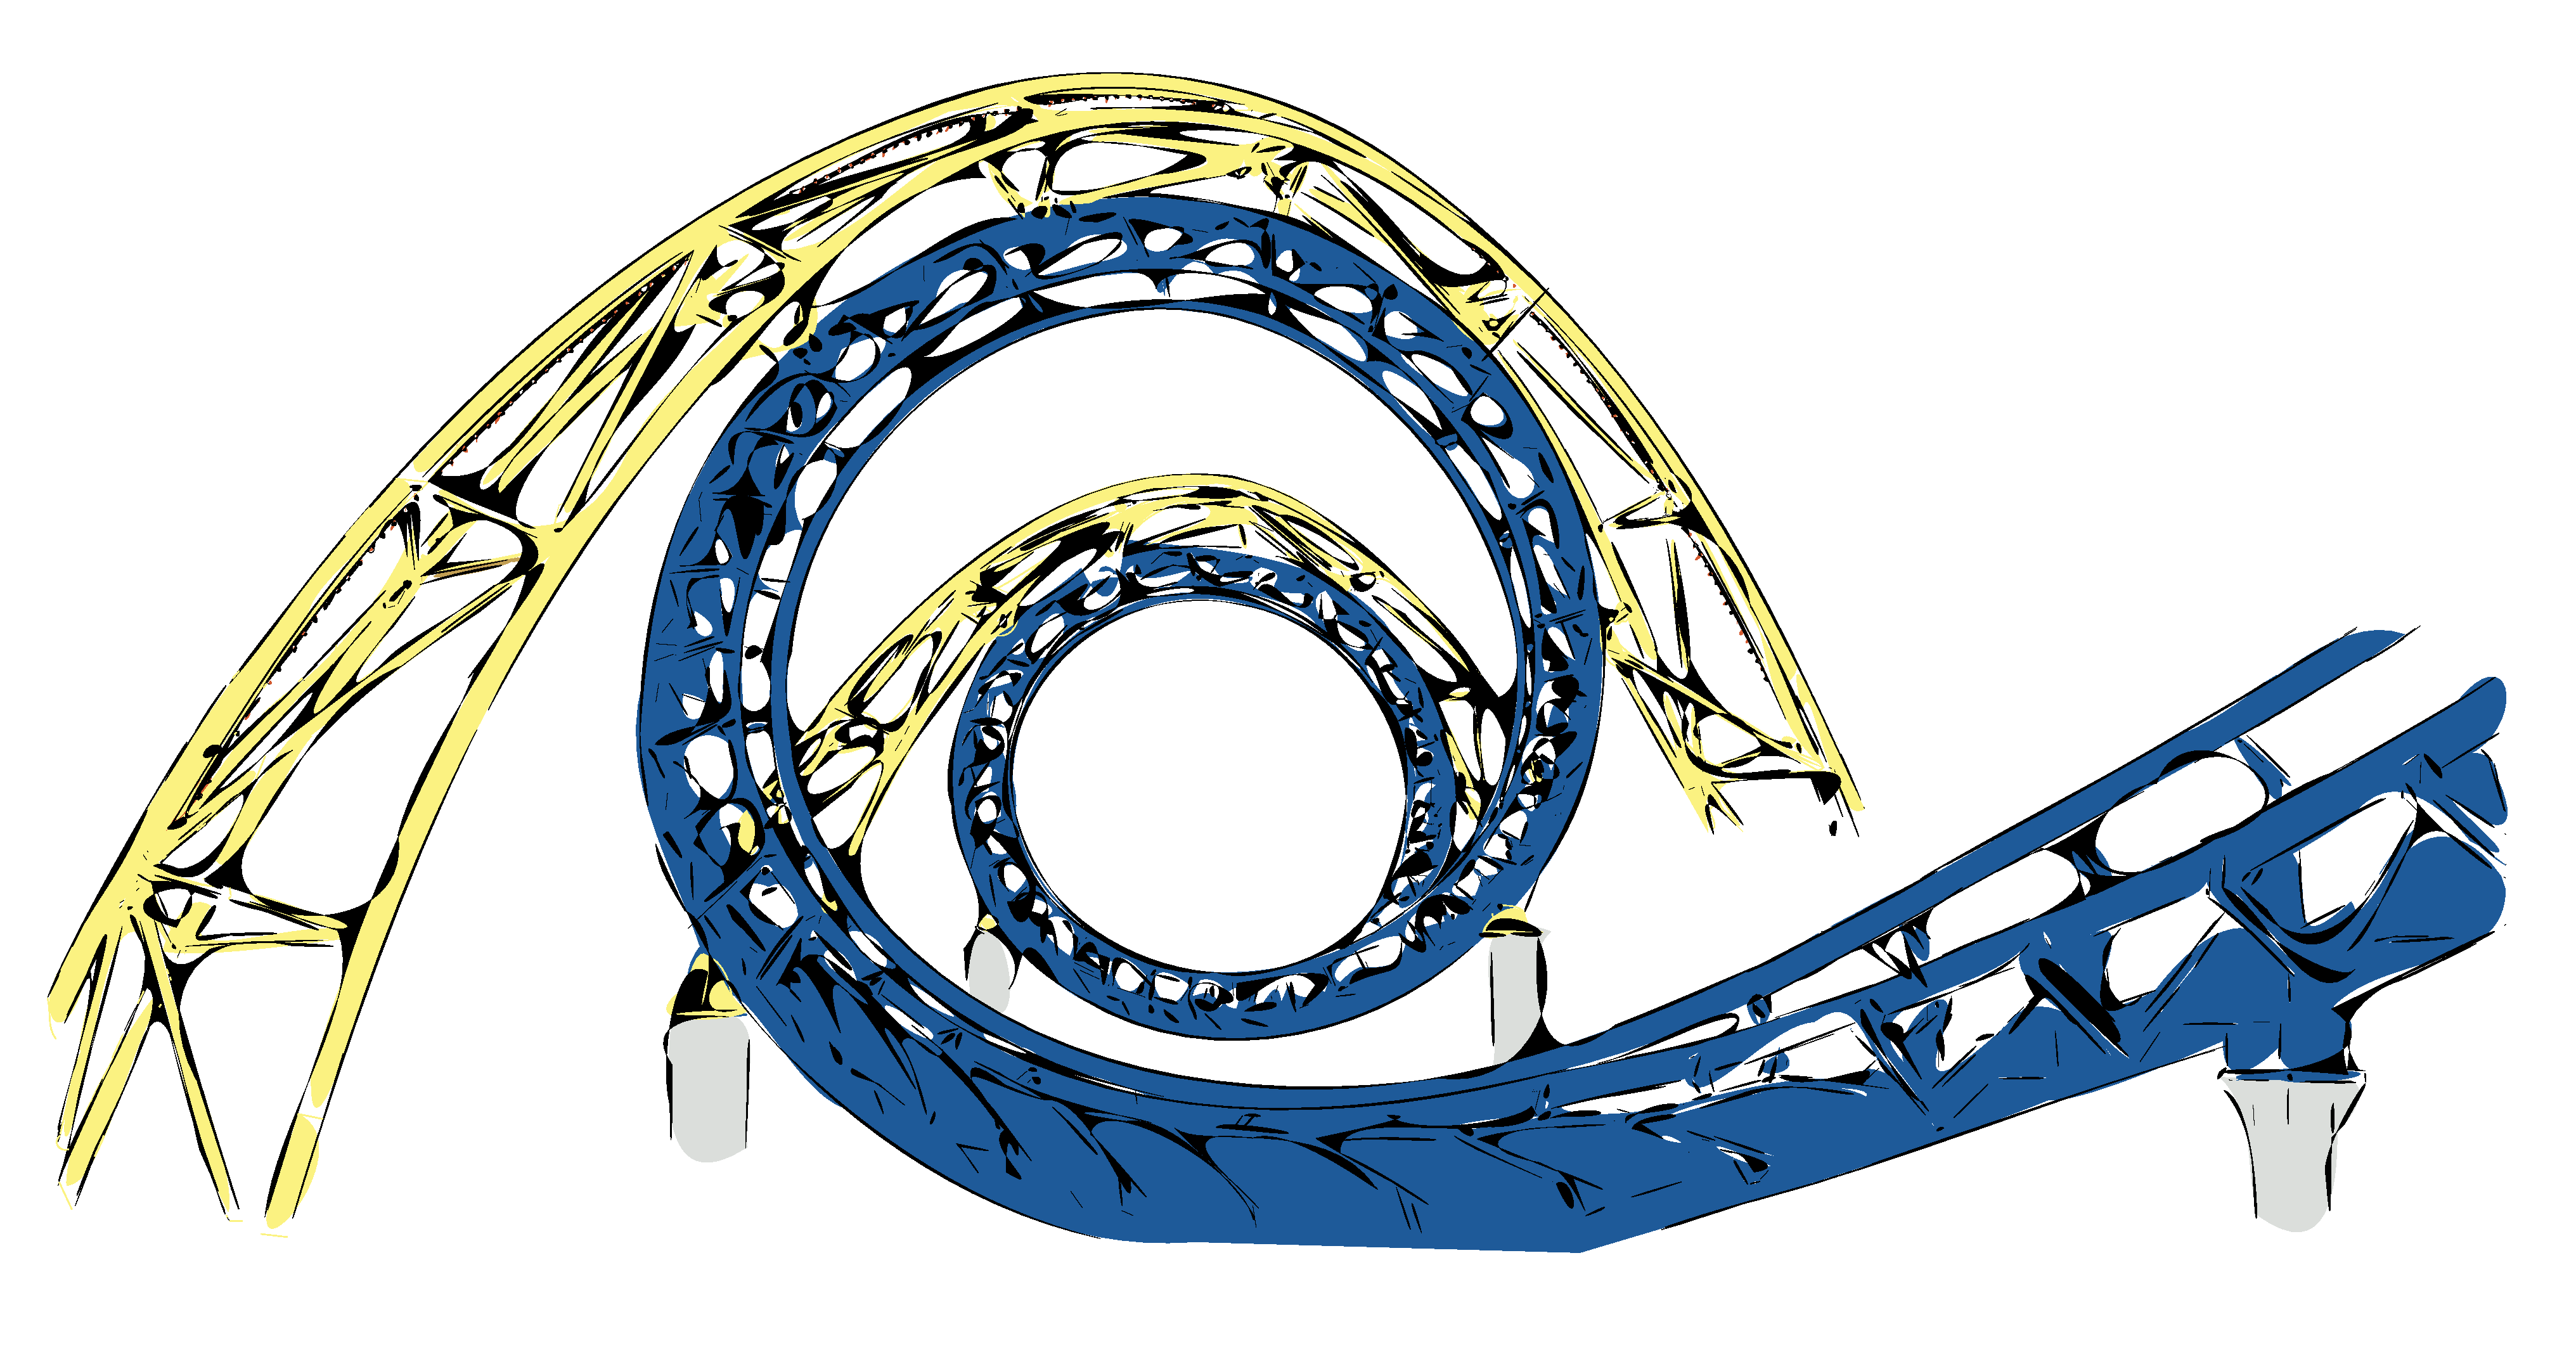
\includegraphics[scale=.2]{images/SteveLambert_Roller_Coaster_Tracks.pdf} 
\end{center}


\section{Quand est-ce qu'un bloc n'est pas compact?}
Quand c'est un bloc de code.\\

Qu'est-ce qu'un «~bloc de code~», alors?\\

Un bloc de code est une série d'instructions que vous voulez grouper ensemble.
Par exemple, dans la boucle ci-dessus vous pourriez avoir envie de faire plus qu'afficher des éléments. 
Peut-être que vous voudriez acheter chaque objet et afficher qu'il l'a bien été.
Supposons que nous avons une fonction appelé «~\texttt{acheter}~» vous pourriez écrire quelque chose comme cela :

\begin{Verbatim}[frame=single,rulecolor=\color{gray}, label=ne pas saisir]
>>> for i in courses :
... 	acheter(i)
... 	print(i)
\end{Verbatim}

Ne vous cassez pas la tête à taper cet exemple dans la console Python car nous n'avons pas de fonction «~\texttt{acheter}~» et que vous auriez un message d'erreur si vous tentiez de la lancer. 
Néanmoins cet exemple permet de montrer un bloc fait de deux commandes:

\begin{Verbatim}[frame=single,rulecolor=\color{gray}, label=ne pas saisir]
acheter(i)
print(i)
\end{Verbatim}

De manière plus utile nous pouvons aussi tracer un cercle avec la tortue sans fonction cercle:

\begin{Verbatim}[frame=single,rulecolor=\color{green}, label=à taper avec attention]
>>> import turtle
>>> tortue=turtle.Pen()
>>> for i in range(360):
...     tortue.forward(1)
...     tortue.left(1)
...
\end{Verbatim}

Vous pouvez observer le résultat sur la figure \ref{fig:cercle}.
\begin{figure}[H]
\centering
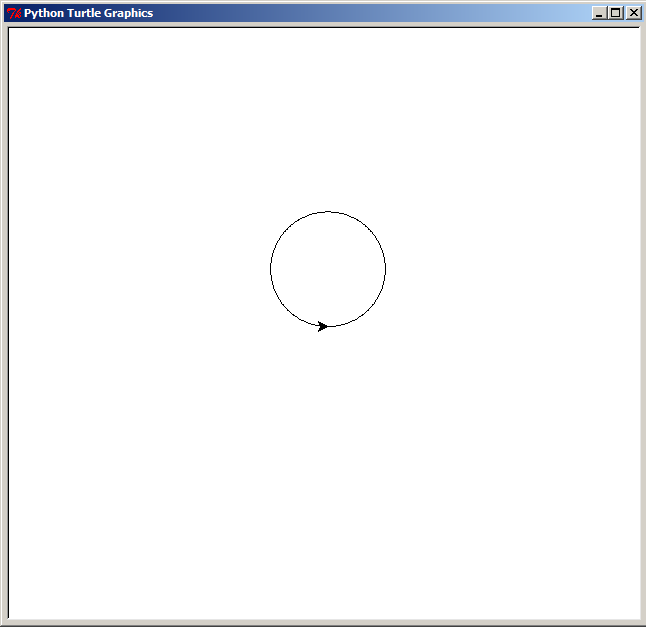
\includegraphics[scale=0.4]{images/cercle.png}
\caption{Un cercle fait en 360 étapes}
\label{fig:cercle}
\end{figure}


En Python, les espaces que ce soient des espaces normales ou des tabulations «~\textsf{⇆}~» sont extrêmement  importantes (bis). Le code qui est positionné à la même position horizontalement est groupé ensemble en blocs.\\


La figure \ref{fig:blocs} montre le découpage en bloc selon la position.
\begin{figure}[H]
\centering
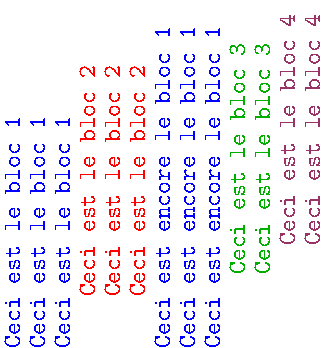
\includegraphics[scale=1,angle=270]{images/blocs.pdf}
\caption{Les blocs en Python}
\label{fig:blocs}
\end{figure}

On commence un nouveau bloc après une ligne finissant   par «~\verb+:+~». Le nouveau bloc est défini par rapport à son indentation (la distance avec le bord gauche). Le bloc initié par «~\verb+:+~» doit avoir une indentation plus grande (être plus à droite) que le bloc précédent.\\


Attention vous devez être cohérents avec vos espacements. Par exemple, nous aurons une erreur avec:

\begin{Verbatim}[frame=single,rulecolor=\color{red}, label=erreur]
>>> for i in courses:
...     acheter(i)
...       print(i)
\end{Verbatim}

La seconde ligne (avec la fonction «~\texttt{acheter(i)}~») commence avec \textbf{quatre} espaces. La troisième ligne commence avec \textbf{six} espaces. Regardons attentivement le code en mettant en valeur les espaces avec des arobases:

\begin{Verbatim}[frame=single,rulecolor=\color{gray}, label=ne pas saisir]
>>> for i in courses:
... @@@@acheter(i)
... @@@@@@print(i)
\end{Verbatim}

Cela causera une erreur. Quand nous commençons un bloc avec quatre espaces vous devez continuer quatre espaces. Et cela tant que vous ne créez pas un nouveau bloc avec «~\verb+:+~» ou que vous ne finissiez pas le bloc en revenant à un niveau d'indentation précédent.\\

Il est d'usage d'indenter les blocs avec des espaces, ou pour le moins, de ne pas mélanger les espaces et les tabulations. De plus on utilise généralement des pas d'indentation constant de quatre espaces.
Si vous commencez un bloc dans un bloc indenté de quatre espaces, il convient d'indenter le nouveau de huit (2x4).
Par exemple, on tapera:

\begin{Verbatim}[frame=single,rulecolor=\color{gray}, label=ne pas saisir]
@@@@un premier bloc
@@@@un premier bloc
@@@@un premier bloc
@@@@@@@@un deuxième bloc
@@@@@@@@un deuxième bloc
@@@@@@@@un deuxième bloc
\end{Verbatim}

Pourquoi allons nous vouloir mettre un bloc «~dans~» un autre? Généralement nous faisons cela quand le deuxième bloc repose sur le premier d'une certaine façon, comme dans une boucle.

Si nous commençons une boucle dans le premier bloc alors les instructions que nous voulons exécuter encore et encore sont dans le second, le second bloc repose sur le premier pour fonctionner correctement.\\

Dans une console Python, une fois que vous commencez à taper du code dans un bloc, Python continue ce bloc jusqu'à ce que vous pressiez entrée sur une ligne vide (ou que vous changez de bloc). Vous pouvez observer trois points au début de chaque ligne qui indiquent que vous continuez à être dans un bloc.\\

Essayons maintenant quelques \emph{vrais} exemples. Ouvrez la console et tapez ce qui suit en vous rappelant de presser la barre d'espace quatre fois au début des lignes qui commencent par «~\texttt{print}~»:

\begin{Verbatim}[frame=single,rulecolor=\color{green}, label=à saisir avec attention]
>>> maliste = [ 'a', 'b', 'c' ]
>>> for i in maliste:
...     print(i)
...     print(i)
...
a
a
b
b
c
c
\end{Verbatim} 

Après le second «~\texttt{print}~» appuyez sur la touche entrée sur la ligne blanche pour dire à la console que vous souhaitez finir le bloc. Cela affichera chaque élément deux fois.\\

L'exemple suivant va créer un message d'erreur:

\begin{Verbatim}[frame=single,rulecolor=\color{red}, label=erreur]
>>> maliste = [ 'a', 'b', 'c' ]
>>> for i in maliste:
...     print(i)
...       print(i)
...
File <stdin>, line 3
print(i)
^
IndentationError: unexpected indent
\end{Verbatim}

La seconde ligne avec «~\texttt{print}~» a six espaces et non quatre sans avoir été introduite par deux points. Python n'aime pas cela car l'indentation doit rester la même au sein d'un même bloc.

\begin{center}

\fcolorbox{black}{lbleu}{
 \begin{minipage}{12cm}
\textbf{Pense-bête}\\

Si vous commencez un bloc de code avec quatre espaces vous devez continuer avec quatres espace. De plus il est conseillé de toujours utiliser des indentations multiples de la première indentation choisie comme 4, 8, 12.

La pluspart des programmeurs Python utilisent des indentations de quatres espaces. Pour faciliter l'éventuelle fusion de code, il est donc conseillé d'utiliser, vous aussi des indentations de quatres espaces.

De plus si vous utilisez IDLE comme éditeur (pas dans le Shell) l'appui sur la touche tabulation «~\textsf{⇆}~» insérera quatres espaces. Le shell IDLE ajoute automatiquement une indentation réalisée avec une tabulation. Le passage d'un bloc à un autre sur une ligne peut être fait en utilisant les flèches horizontales.

\end{minipage}
 }
\end{center}



Vois un exemple qui met en œuvre deux blocs de code:

\begin{Verbatim}[frame=single,rulecolor=\color{gray}, label=ne pas saisir]
>>> maliste = [ 'a', 'b', 'c' ]
>>> for i in maliste:
...     print(i)
...     for j in maliste:
...         print(j)
...
\end{Verbatim}

Où sont les blocs dans ce code que va-t-il faire?
Il a deux blocs, le premier fait parti de la première boucle:

\begin{Verbatim}[frame=single,rulecolor=\color{gray}, label=ne pas saisir]
>>> maliste = [ 'a', 'b', 'c' ]
>>> for i in maliste:
...     print(i)              # Ces deux lignes sont
...     for j in maliste:     # le premier bloc
...         print(j)
...
\end{Verbatim}

Le deuxième bloc est la ligne «~\texttt{print}~» solitaire dans la seconde boucle:

\begin{Verbatim}[frame=single,rulecolor=\color{gray}, label=ne pas saisir]
>>> maliste = [ 'a', 'b', 'c' ]
>>> for i in maliste:
...     print(i) 
...     for j in maliste:
...         print(j)          # Second bloc
...
\end{Verbatim}

Au passage vous pouvez observer des dièses «~\texttt{\#}~» qui sont utilisés pour marquer des commentaires. Les commentaires sont du texte qui n'est pas pris en compte pour l'éxécution mais qui apporte des informations sur le code et permettent de le documenter (pour un usage ultérieur par exemple).\\


Pouvez-vous déduire ce que ce petit bout de code va faire?
Il va afficher les trois lettres de «~\texttt{maliste}~», mais combien de fois?
Si nous étudions chaque ligne nous pouvons probablement trouvez ce nombre de fois.
Nous savons que la première boucle va parcourir tous les objets de la liste et exécuter
les commandes du premier bloc. Donc elle va afficher une lettre puis lancer la seconde boucle. Cette boucle va elle aussi parcourir les éléments de la liste et exécuter les commandes du deuxième bloc. Ainsi nous pouvons comprendre ce qui est affiché quand le code est exécuté, ce sera un «~\texttt{a}~»  suivi de «~\texttt{a}~», «~\texttt{b}~», «~\texttt{c}~» puis un «~\texttt{b}~»  suivi de «~\texttt{a}~», «~\texttt{b}~», «~\texttt{c}~» et ainsi de suite.\\

Entre le code dans console et voyez par vous-même:

\begin{Verbatim}[frame=single,rulecolor=\color{green}, label=à saisir avec attention]
>>> maliste = [ 'a', 'b', 'c' ]
>>> for i in maliste:
...     print(i)
...     for j in maliste:
...         print(j)
...
a
a
b
c
b
a
b
c
c
a
b
c
\end{Verbatim}

Et si nous faisions maintenant quelque chose de plus utile que juste afficher des lettres?
Rappelez-vous les calculs que nous avions fait au début de ce livre sur les économies que vous pourriez réaliser. Il s'agissait de calculer les économies si vous gagniez 10\begin{small}\euro\end{small} par semaine en faisant le ménage, 30\begin{small}\euro\end{small} en distribuant le journal et vous dépensiez 10\begin{small}\euro\end{small}.\\

Cela ressemblait à cela:

\begin{Verbatim}[frame=single,rulecolor=\color{gray}, label=ne pas saisir]
>>> (5 + 30 - 10) * 52
\end{Verbatim}

C'est à dire 5\begin{small}\euro\end{small}+30\begin{small}\euro\end{small}-10\begin{small}\euro\end{small} multiplié par 52 semaines dans l'année.\\

Il pourrait être utile de voir de combien vos économies augmentent durant l'année plutôt que de savoir ce qu'elles seront en toute fin d'année. Nous pouvons calculer cela avec un itérateur. Mais premièrement nous devonc mettre ces nombres dans des variables:

\begin{Verbatim}[frame=single,rulecolor=\color{mbleu}, label=à taper]
>>> ménage = 5
>>> journaux = 30
>>> dépenses = 10
\end{Verbatim}

Nous pouvons faire le calcul original en utilisant ces variables:

\begin{Verbatim}[frame=single,rulecolor=\color{mbleu}, label=à taper]
>>> (ménage + journaux - dépenses) * 52
1300
\end{Verbatim}

Ou nous pouvons voir nos économies augmenter au cours de l'année en créant une autre variable appelée «~\texttt{économies}~» et l'utiliser dans une boucle:

\begin{Verbatim}[frame=single,rulecolor=\color{mbleu}, label=à taper]
>>> économies=0
>>> for semaine in range(1, 53):
...     économies = économies + ménage + journaux - dépenses
...     print('Semaine %s = %s€' % (semaine,économies))
... 
\end{Verbatim}

À la première ligne la variable «~\texttt{économies}~» est créée avec pour valeur zéro car nous n'avons encore
rien économisé. Si nous ne créons pas cette variable nous ne pourons pas dire à la première étape que les économie de la première semaine sont égales à celles d'avant qu'on débute. On pourrait écrire:

\begin{Verbatim}[frame=single,rulecolor=\color{gray}, label=moche]
>>> économies=économies + ménage + journaux - dépenses
>>> for semaine in range(2, 53):
...     économies = économies + ménage + journaux - dépenses
...     print('Semaine %s = %s€' % (semaine,économies))
... 
\end{Verbatim}

Mais cela ferait du code à taper en plus, pour rien.\\

\emph{Les bons programmeurs ne tapent pas du code pour rien.}\\



La deuxième ligne commence un itérateur (une boucle) qui va exécuter les commandes dans le bloc constitué de la troisième et de la quatrième ligne. À chaque itération (à chaque tour de la boucle) la variable «~\texttt{semaine}~» est chargée avec le nombre suivant de la série 1 à 52.

La troisième ligne est un peu plus compliquée. Simplement, pour chaque semaine nous voulons ajouter ce que nous avons économisé à nos «~\texttt{économies}~» totales. Pensez à la variable «~\texttt{économie}~» comme à une tirelire. En langage Python la troisième ligne veut dire: remplace le contenu de la variable «~\texttt{économies}~» par mes économies actuelles plus ce que j'ai gagné cette semaine.

Le symbole «~\texttt{=}~» est un bout de code astucieux pour dire: calcule ce qu'il y a à droite en premier puis garde le pour plus tard en utilisant le nom qui est à gauche.\\

Si la ligne contenant «~\texttt{économie=économie+...}~» vous semble trop difficile à comprendre, sachez que l'on peut aussi écrire:

\begin{Verbatim}[frame=single,rulecolor=\color{mbleu}, label=à taper]
>>> économies=0
>>> for semaine in range(1, 53):
...     économies += ménage + journaux - dépenses
...     print('Semaine %s = %s€' % (semaine,économies))
... 
\end{Verbatim}

C'est à dire ajouter à «~\texttt{économie}~» le résultat de «~\texttt{ménage + journaux - dépenses}~». La quatrième ligne est une instruction «~\texttt{print}~» légèrement compliquée. Elle affiche le numéro de la semaine et le montant total des économies réalisé pour cette semaine. Si cette ligne n'a pas beaucoup de sens pour vous rafraichissez vos connaissances sur les chaînes en consultant la \autoref{sec:tours} «~Tours de chaînes~»  page \pageref{sec:tours}.

Si vous exécutez le programme vous aurez comme résultat:

\begin{Verbatim}[frame=single,rulecolor=\color{gray}, label=ne pas saisir]
Semaine 1 = 25€
Semaine 2 = 50€
Semaine 3 = 75€
Semaine 4 = 100€
Semaine 5 = 125€
Semaine 6 = 150€
[...]
Semaine 49 = 1225€
Semaine 50 = 1250€
Semaine 51 = 1275€
Semaine 52 = 1300€
\end{Verbatim}

\section{Tant que nous en sommes à parler de boucles...}

L'itérateur n'est pas la seule sorte de boucle que nous pouvons faire en Python.  Il y a aussi une boucle «~tant que~». Alors que dans le cas d'un itérateur nous savons exactement quand nous allons sortir de la boucle, dans une boucle «~tant que~» nous ne savons pas forcément quand nous allons sortir de la boucle.  Imaginez un escalier avec vingt marches. Vous savez que vous pouvez facilement monter vingt marches, vous pouvez employer un itérateur.

\begin{Verbatim}[frame=single,rulecolor=\color{gray}, label=ne pas saisir]
>>> for marche in range(0,20):
...     print(marche)
\end{Verbatim}

Maintenant imaginons que l'escalier permet de monter en haut d'une montagne. Vous pouvez être épuisé avant d'atteindre le sommet. Ou les conditions météorologiques peuvent devenir mauvaises vous obligeant à vous arrêter.
C'est une boucle «~tant que~».

\begin{Verbatim}[frame=single,rulecolor=\color{gray}, label=ne pas saisir]
>>> marche = 0
>>> continuer=True
>>> while continuer :
...     print(marche)
... 	if marche==10000
...         continuer=False
...     elif fatigué():
...         continuer=False
...     elif mauvais_temps():
...         continuer=False
...     else:
...         marche += 1
\end{Verbatim}

Ne vous ennuyez pas à taper l'exemple ci-dessous car nous ne nous sommes pas ennuyés à créer les fonctions «~\texttt{fatigué()}~» et «~\texttt{mauvais\_temps()}~» 

Le mot \emph{while} signifie «~tant que~» en anglais, \emph{True} signifie «~vrai~» et \emph{False} signifie «~faux~».

Cet exemple montre les bases d'une d'une boucle tant que. Tant que «~\texttt{continuer}~» est vrai le bloc de code sera exécuté. Dans le bloc nous affichons la valeur de «~\texttt{marche}~» puis nous vérifions si nous sommes arrivés «~\texttt{marche==1000}~», si nous sommes fatigués ou si le temps est mauvais.

Les boucles tant que peuvent être représentées comme sur la figure \ref{fig:Cf-while-fr}.
\begin{figure}[h!]
\centering
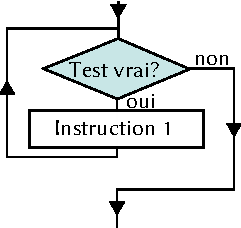
\includegraphics[scale=1.5]{images/Cf-while-fr.pdf}
\caption{Diagramme d'une boucle tant que}
\label{fig:Cf-while-fr}
\end{figure}

Cet algorithme\footnote{Un algorithme est un ensemble d'opérations ordonné qui permet de réaliser une opération plus complexe.} peut aussi être écrit\footnote{Ces exemples se veulent didactiques, nous verrons plus tard comment ces écritures peuvent être condensées.}:

\begin{Verbatim}[frame=single,rulecolor=\color{gray}, label=ne pas saisir]
>>> marche = 0
>>> while marche < 10001:
...     print(step)
...     if fatigué():
...         break
...     elif mauvais_temps():
...         break
...     else:
...         marche = marche + 1 
\end{Verbatim}

Tant que «~\texttt{marche}~» vaut moins de 10001 (tant que nous ne sommes pas arrivés) le bloc de code sera exécuté. Dans le bloc nous affichons la valeur de «~\texttt{marche}~» puis nous vérifions si nous sommes fatigués ou si le temps est mauvais. Si c'est le cas l'instruction «~\texttt{break}~» nous fait sortir de la boucle (nous sautons hors de la boucle à la ligne qui suit le bloc). Sinon nous ajoutons un à marche puis la condition de la boucle est contrôlée à nouveau.

Le mot \emph{break} signifie casser en anglais, \emph{break out}, s'évader.\\


Les étapes d'une boucle «~tant que~» sont simplement:
\begin{itemize}
\item vérifier la condition;
\item exécuter le code dans le bloc;
\item répéter.
\end{itemize}

Le plus souvent, une boucle tant que prendra en compte plusieurs conditions à la fois:

\begin{Verbatim}[frame=single,rulecolor=\color{gray}, label=ne pas saisir]
>>> marche = 0
>>> while marche < 10001 and en_forme() and beau_temps():
...     print(step)
...     marche = marche + 1 
\end{Verbatim}

Ou moins imagé mais que vous pouvez saisir tout de suite:

\begin{Verbatim}[frame=single,rulecolor=\color{mbleu}, label=à taper]
>>> x = 45
>>> y = 80
>>> while x < 50 and y < 100:
...     x = x + 1
...     y = y + 1
...     print(x, y)
\end{Verbatim}

Avant cette boucle nous créons une variable «~\texttt{x}~»  initialisé à 45 et une variable «~\texttt{y}~» initialisé à 80. Deux conditions doivent être vraies pour que le bloc de la boucle soit exécuté: x vaut moins de 50 et y moins de 100. Tant que les deux conditions sont vraies le bloc de code est exécuté. Ce bloc ajoute un aux deux variables et les affiche. Le résultat est juste:

\begin{Verbatim}[frame=single,rulecolor=\color{gray}, label=ne pas saisir]
46 81
47 82
48 83
49 84
50 85
\end{Verbatim}

Peut-être vous demandez-vous pourquoi ces nombres et seulement ces nombres sont imprimés?\\

Nous commençons à compter à partir de 45 pour «~\texttt{x}~»  et de 80 pour «~\texttt{y}~». Puis nous incrémentons (ajoutons un) à chaque variable à chaque «~tour~» de boucle. Le contrôle des conditions vérifie que x fait moins de 50 et y fait moins de 100. Après avoir parcouru la boucle cinq fois (en ajoutant un à chaque variable) la valeur de x atteint cinquante. Maintenant la première condition «~\texttt{x < 50}~»  est fausse donc Python arrête de boucler.

Un autre usage courant des boucle tant que est de créer des boucles semi-éternelles. 
Il s'agit de boucles qui s'exécutent pour toujours ou du moins jusqu'à ce quelque chose arrive dans le code qui va l'arrêter. Par exemple:

\begin{Verbatim}[frame=single,rulecolor=\color{gray}, label=ne pas saisir]
>>> while True:
...     plein de code ici
...     plein de code ici
...     plein de code ici
...     if une_condition == True:
...         break
\end{Verbatim}

La condition pour cette boucle tant que est juste «~\texttt{True}~» (vrai). Ainsi le code du bloc va toujours s'exécuter (c'est pourquoi la boucle est dite éternelle ou infinie). Néanmoins, si la variable «~\texttt{une\_condition}~»   devient vraie alors le code sortira de la boucle grâce à l'instruction «~\texttt{break}~». Vous trouverez un meilleur exemple de ce type de boucle infinie dans l'annexe C (dans la section à propos du module «~\texttt{random}~»  ) mais vous devriez attendre d'avoir lu le prochain chapitre avant d'y jeter un coup d'œil.

\section{À vous de jouer\label{PRATIQUE:BOUCLES}}
Dans ce chapitre nous avons vu comment utiliser des boucles pour réaliser des actions répétitives. Nous avons utilisé des blocs de code à l'intérieur de boucle pour les taches à répéter.


Vous trouverez des pistes de réponses dans la \autoref{REPONSES:BOUCLES}.
\subsection{Exercice 1}
Que pensez vous qu'il va arriver avec le code suivant?
\begin{Verbatim}[frame=single,rulecolor=\color{mbleu}, label=à taper]
>>> for x in range(0, 20):
... 	print('x vaut %s' % x)
... 	if x < 9:
... 		break
\end{Verbatim}

\subsection{Exercice 2}
Un lac est envahi par des nénuphars issus d'un jardin. Le premier jour un seul nénuphar est présent dans le lac.
Tous les jours le nombre de nénuphars double (est multiplié par deux). 
Sachant que le lac sera complètement envahi quand il y aura plus de mille nénuphars, combien de jours faut-il pour arriver à ce stade?

 \vfill
\begin{center}
 
\includegraphics[width=5cm]{images/sem2.pdf}
\end{center}
 \vfill

%\newpage
 
% \AddToShipoutPicture*{
% \put(0,0){
% \parbox[b][\paperheight]{\paperwidth}{

% }}}
\clearemptydoublepage